% -*- latex -*-
%%%%%%%%%%%%%%%%%%%%%%%%%%%%%%%%%%%%%%%%%%%%%%%%%%%%%%%%%%%%%%%%
%%%%%%%%%%%%%%%%%%%%%%%%%%%%%%%%%%%%%%%%%%%%%%%%%%%%%%%%%%%%%%%%
%%%%
%%%% This text file is part of the source of 
%%%% `Parallel Programming in MPI and OpenMP'
%%%% by Victor Eijkhout, copyright 2012-6
%%%%
%%%% mpi-blocksend.tex : blocking sends
%%%%
%%%%%%%%%%%%%%%%%%%%%%%%%%%%%%%%%%%%%%%%%%%%%%%%%%%%%%%%%%%%%%%%
%%%%%%%%%%%%%%%%%%%%%%%%%%%%%%%%%%%%%%%%%%%%%%%%%%%%%%%%%%%%%%%%

\Level 0 {Blocking point-to-point operations}

Suppose you have an array of numbers $x_i\colon i=0,\ldots,N$
and you want to compute $y_i=(x_{i-1}+x_i+x_{i+1})/3\colon i=1,\ldots,N-1$.
As before (see figure~\ref{fig:mpi-array}), we give each processor
a subset of the~$x_i$s and $y_i$s.
Let's define $i_p$ as the first index of~$y$ that is
computed by processor~$p$. (What is the last index computed by processor~$p$?
How many indices are computed on that processor?)

We often talk about the \indexterm{owner computes}
model of parallel computing: each processor `owns' certain data items,
and it computes their value.

Now let's investigate how processor~$p$ goes about computing~$y_i$ for
the $i$-values it owns. Let's assume that processor~$p$ also stores
the values $x_i$ for these same indices.
Now, it can compute
\[ y_{i_p+1} = (x_{i_p}+x_{i_p+1}+x_{i_p+2})/3 \]
and likewise $y_{i_p+2}$ and so on. However, there is a problem with
\[ y_{i_p} = (x_{i_p-1}+x_{i_p}+x_{i_p+1})/3 \]
since $x_{i_p}$ is not stored on processor~$p$: it is stored on~$p-\nobreak1$.

There is a similar story with the last index that $p$ tries to compute:
that involves a value that is only present on~$p+1$.

You see that there is a need for processor-to-processor, or
technically \indexterm{point-to-point}, information exchange.
MPI realizes this through matched send and receive calls:
\begin{itemize}
\item One process does a send to a specific other process;
\item the other process does a specific receive from that source.
\end{itemize}

\Level 1 {Send example: ping-pong}

A simple scenario for information exchange between just two processes
is the \indexterm{ping-pong}: process~A sends data to process~B, which
sends data back to~A. This means that process~A executes the code
\begin{verbatim}
MPI_Send( /* to: */ B ..... );
MPI_Recv( /* from: */ B ... );
\end{verbatim}
while process~B executes
\begin{verbatim}
MPI_Recv( /* from: */ A ... );
MPI_Send( /* to: */ A ..... );
\end{verbatim}
Since we are programming in SPMD mode, this means our program looks like:
\begin{verbatim}
if ( /* I am process A */ ) {
  MPI_Send( /* to: */ B ..... );
  MPI_Recv( /* from: */ B ... );
} else if ( /* I am process B */ ) {
  MPI_Recv( /* from: */ A ... );
  MPI_Send( /* to: */ A ..... );
}
\end{verbatim}

The blocking send command:
%
\mpiRoutineRef{MPI_Send}
%
This routine may not blocking for small messages; to force blocking
behaviour use \n{MPI_Ssend} with the same argument list.
\url{http://www.mcs.anl.gov/research/projects/mpi/www/www3/MPI_Ssend.html}

The basic blocking receive command:
%
\mpiRoutineRef{MPI_Recv}
%
The \n{count} argument indicates the maximum length of a message; the
actual length of the received message can be determined 
from the status object. See section~\ref{ref:mpi-source}
for more about the status object.

\begin{exercise}
  \label{ex:pingpong}
  Implement the ping-pong program. Add a timer using \n{MPI_Wtime}.
  For the \n{status} argument of the receive call, use
  \indexmpishow{MPI_STATUS_IGNORE}.

  \begin{itemize}
  \item Run multiple ping-pongs (say a thousand) and put the timer
    around the loop. The first run may take longer; try to discard it.
  \item Run your code with the two communicating processes first on
    the same node, then on different nodes. Do you see a difference?
  \item Then modify the program
    to use longer messages. How does the timing increase with message size?
  \end{itemize}
  For bonus points, can you do a regression to determine~$\alpha,\beta$?
\end{exercise}

\begin{exercise}
  \label{ex:hbwpingpong}
  Take your pingpong program and modify it 
  to let half the processors
  be source and the other half the targets. Does the pingpong time increase?
\end{exercise}

In the syntax of the \indexmpishow{MPI_Recv} command you saw one parameter that
the send call lacks: the \indexmpishow{MPI_Status} object. This serves the following
purpose: the receive call can have a `wildcard' behaviour, for instance specifying
that the message can come from any source rather than a specific one. The status
object then allows you to find out where the message actually came from.

\begin{exercise}
  \label{ex:gaussjordan}
  The \indexterm{Gauss-Jordan method} for \indextermsub{solving a}{linear system} or
  computing a \indextermbus{matrix}{inverse} applies the following
  transformations to a matrix:
  \begin{tabbing}
    for \=$k=1,\ldots,n$\\
    \>fin\=d pivot:\\
    \>\> $p=1/a_{kk}$\\
    \>scale rows by the pivot:\\
    \>\> for \=$r=1,\ldots,n$\\
    \>\>\> $a_{rk} = a_{rk}\cdot p$\\
    \>sweep columns:\\
    \>\>\> for \=$c=1,\ldots,n$\\
    \>\>\>\> $a_{rc} = a_{rc} - a_{rk}\cdot a_{kc}$\\
  \end{tabbing}
  (Depending on whether the method is used for a linear system or an
  inverse, we use some form of \indextermsub{augmented}{matrix}.)

  Explore how to parallelize this algorithm if every processor stores
  one column of the matrix. Use blocking send and receive calls.
\end{exercise}

\Level 1 {Problems with blocking communication}
\label{sec:blocking}
\index{communication!blocking|(textbf}

The use of \indexmpishow{MPI_Send} and \indexmpishow{MPI_Recv}
is known as \emph{blocking communication}: when your code reaches a
send or receive call, it blocks until the call is succesfully completed.
For a receive call it is clear that the receiving code will wait until
the data has actually come in, but for a send call this is more subtle.

You may be tempted to think that the send call puts the data somewhere
in the network, and the sending code can progress,
as in figure~\ref{fig:send-ideal}, left.
%
\begin{figure}[ht]
\leavevmode
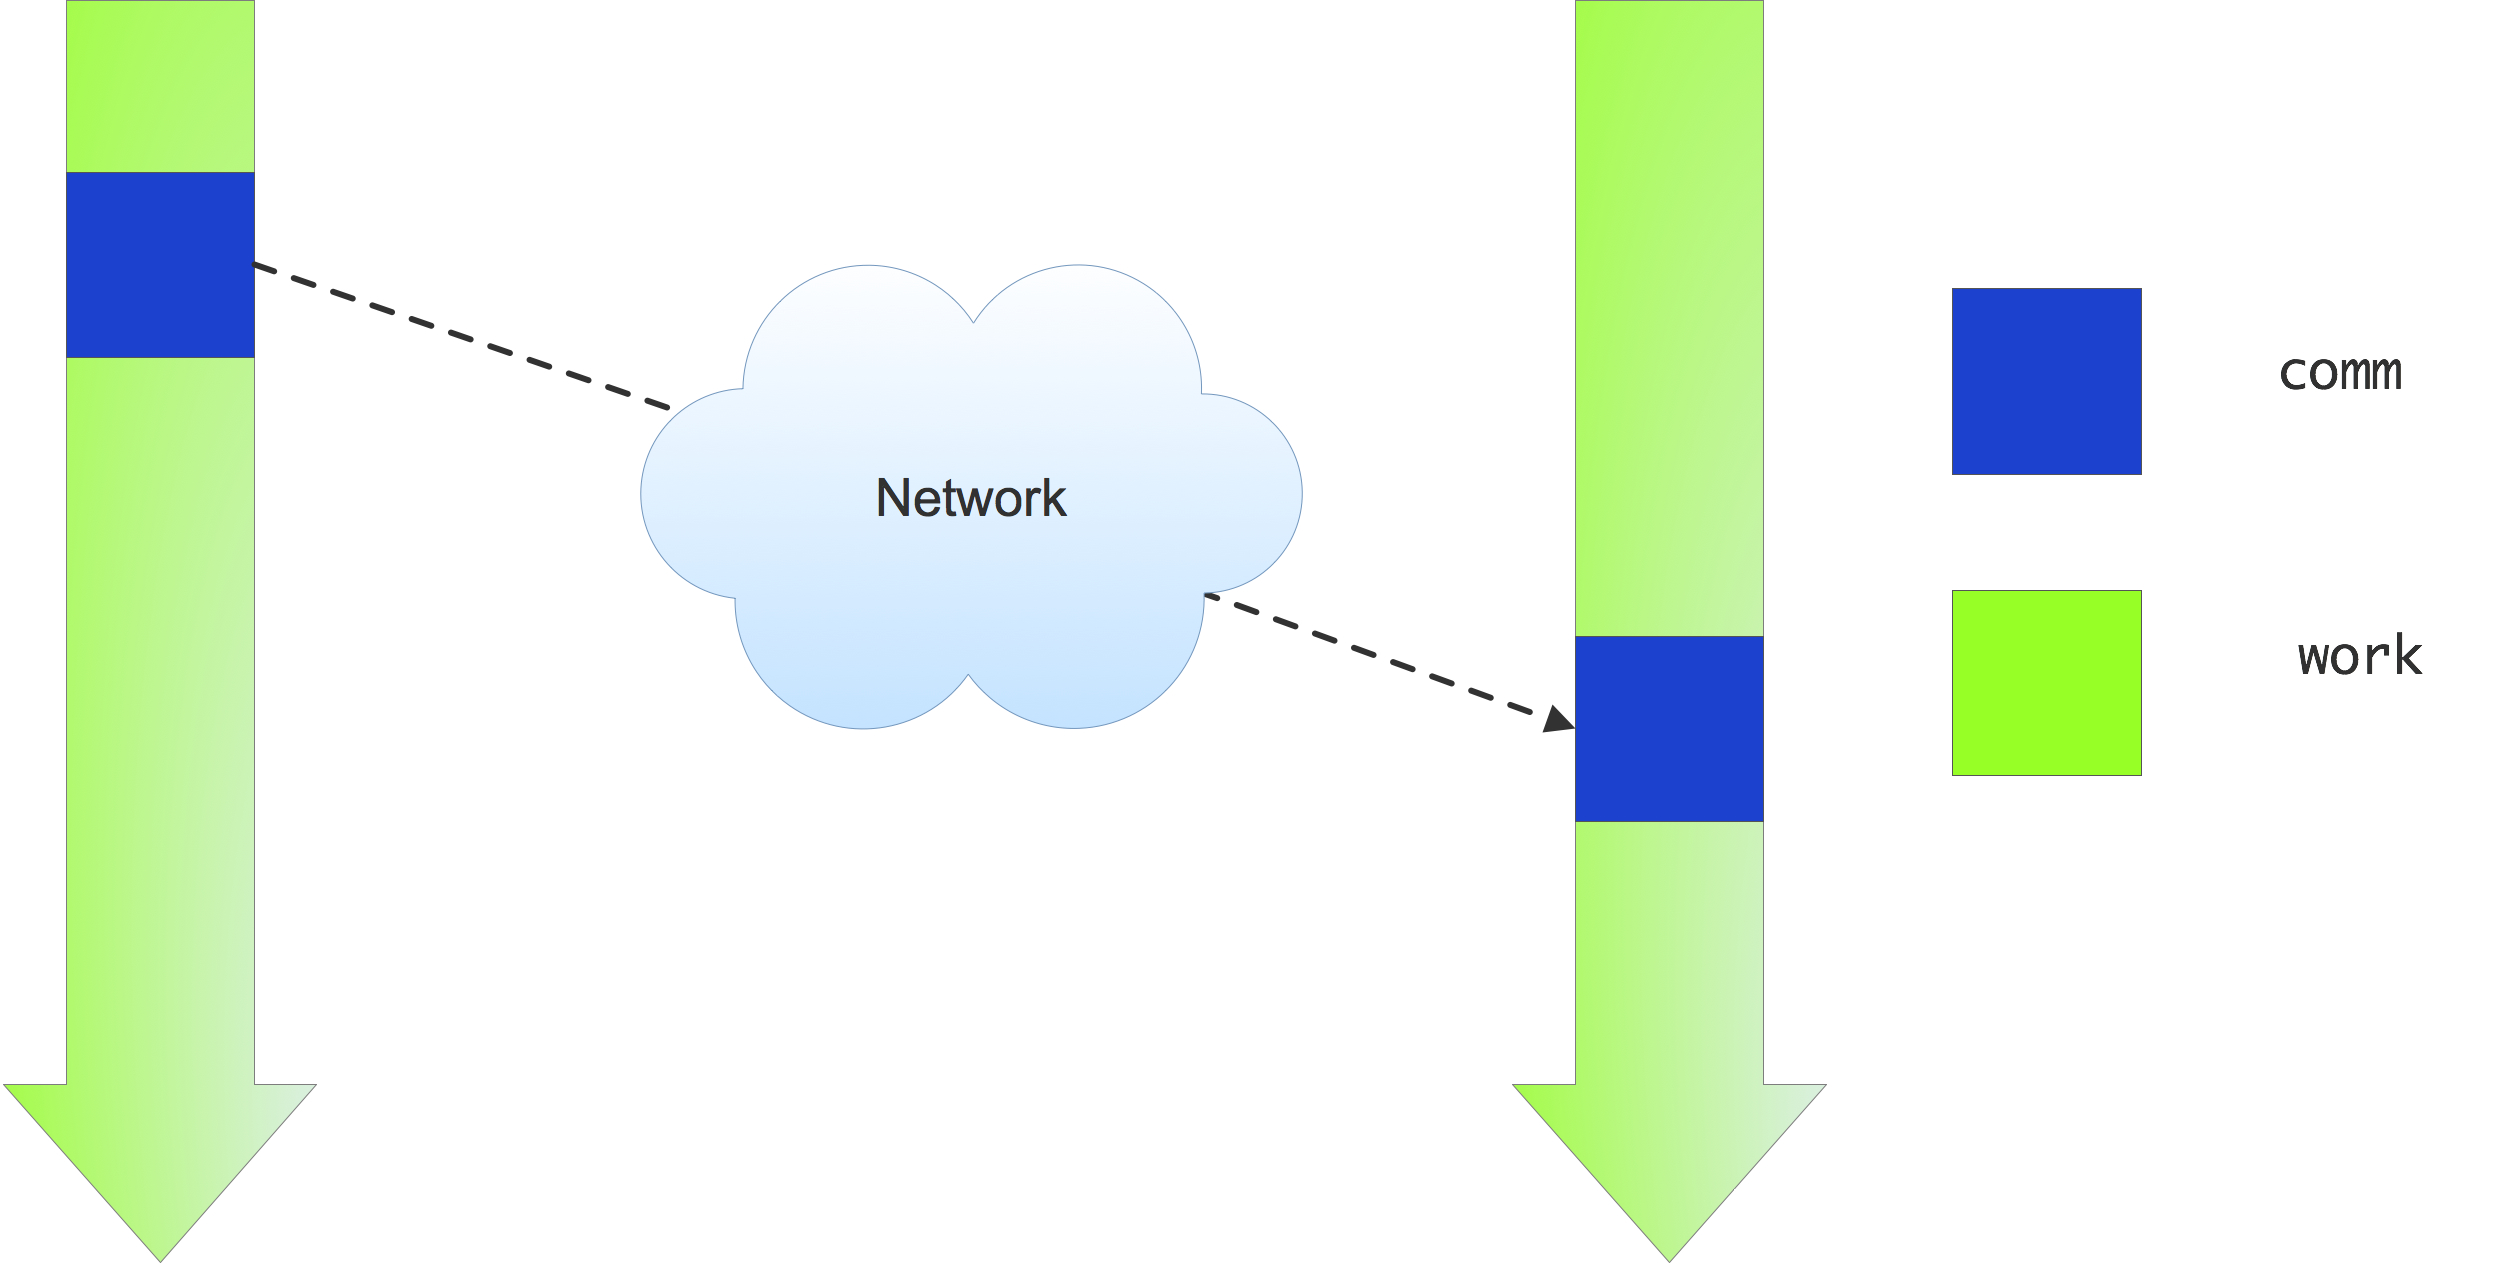
\includegraphics[scale=.08]{graphics/send-ideal}
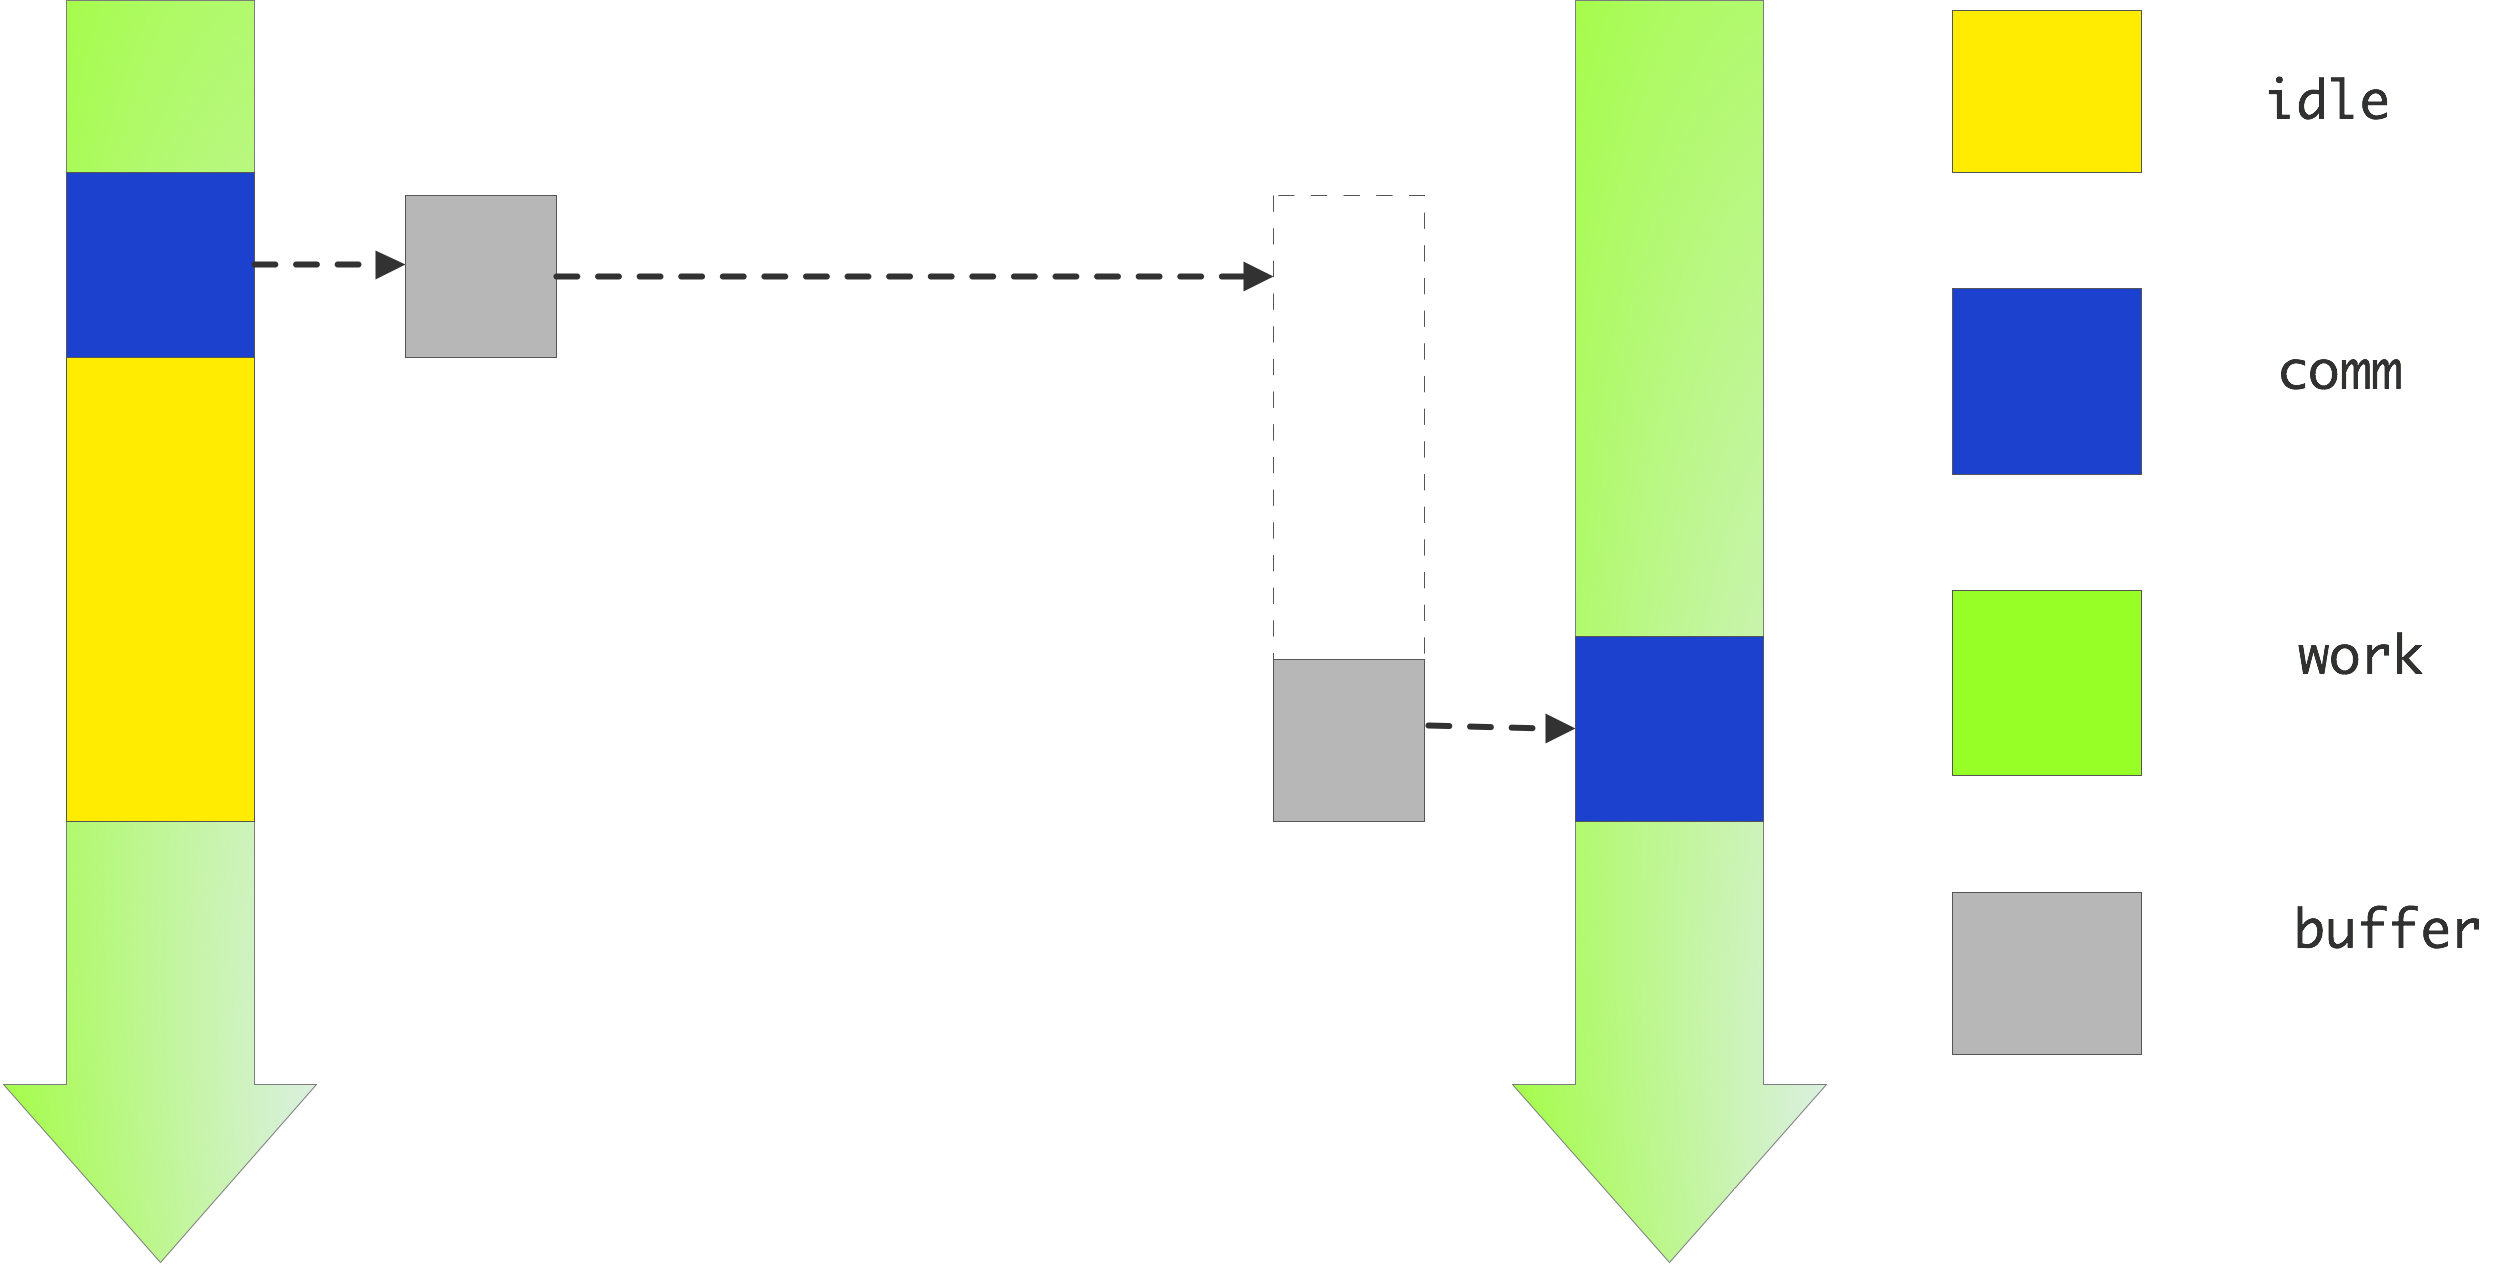
\includegraphics[scale=.08]{graphics/send-blocking}
\caption{Illustration of an ideal (left) and actual (right) send-receive interaction}
\label{fig:send-ideal}
\end{figure}
%
But this ideal scenario is not realistic: it assumes that somewhere
in the network there is buffer capacity for all messages that are in
transit.
This is not the case: data resides on the sender, and the sending call blocks,
until the receiver has received all of it. (There is a exception for
small messages, as explained in the next section.)

\Level 2 {Deadlock}

Suppose two process need to exchange data, and consider the following
pseudo-code, which purports to exchange data between processes 0 and~1:
\begin{verbatim}
other = 1-mytid; /* if I am 0, other is 1; and vice versa */
receive(source=other);
send(target=other);
\end{verbatim}
Imagine that the two processes execute this code. They both issue the
send call\ldots\ and then can't go on, because they are both waiting
for the other to issue a receive call. This is known
as \indextermdef{deadlock}.

(If you reverse the send and receive call, you should get deadlock,
but in practice that code will often work. The reason is that
MPI implementations sometimes send small messages regardless of whether
the receive has been posted. This relies on the availability of
some amount of available buffer space. The size under which this behaviour
is used is sometimes referred to as the \indexterm{eager limit}.)

The following code is guaranteed to block, since a \n{MPI_Recv}
always blocks:
\verbatimsnippet{recvblock}
On the other hand, if we put the send call before the receive,
code may not block for small messages
that fall under the \indexterm{eager limit}.

In this example we send
gradually larger messages. From the screen output you can see what
the largest message was that fell under the eager limit; after that the code
hangs because of a deadlock.
%
\verbatimsnippet{sendblock}
%
\verbatimsnippet{sendblock-f}
%
\verbatimsnippet{sendblockp}


If you want a code to behave the same for all message sizes,
you force the send call to be blocking by using \n{MPI_Ssend}:
\verbatimsnippet{ssendblock}
Formally you can describe deadlock as follows. Draw up a graph where
every process is a node, and draw a directed arc from process~A to~B if
A is waiting for~B. There is deadlock if this directed graph has a
loop.

The solution to the deadlock in the above example
is to first do the send from 0 to~1, and then from 1 to~0 (or the other way around). So the code would look like:
\begin{verbatim}
if ( /* I am processor 0 */ ) {
  send(target=other);
  receive(source=other);
} else {
  receive(source=other);
  send(target=other);
}
\end{verbatim}

\Level 2 {Serialization}

There is a second, even more subtle problem with blocking
communication. Consider the scenario where every processor needs to
pass data to its successor, that is, the processor with the next
higher rank. The basic idea would be to first send to your successor,
then receive from your predecessor. Since the last processor does not
have a successor it skips the send, and likewise the first processor
skips the receive. The pseudo-code looks like:
\begin{verbatim}
successor = mytid+1; predecessor = mytid-1;
if ( /* I am not the last processor */ )
  send(target=successor);
if ( /* I am not the first processor */ )
  receive(source=predecessor)
\end{verbatim}
This code does not deadlock. All processors but the last one block on
the send call, but the last processor executes the receive call. Thus,
the processor before the last one can do its send, and subsequently
continue to its receive, which enables another send, et cetera.

In one way this code does what you intended to do:
it will terminate (instead of hanging forever on a
deadlock) and exchange data the right way. However, the execution
now suffers from unexpected \indexterm{serialization}: only
one processor is active at any time, so what should have been a
%
\begin{figure}[ht]
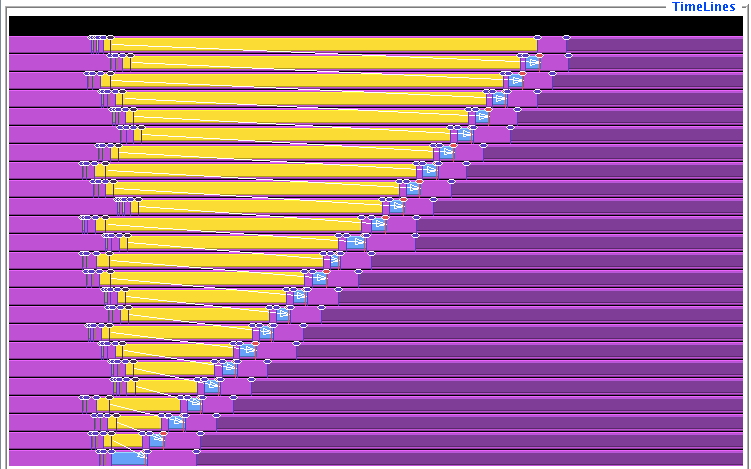
\includegraphics[scale=.4]{graphics/linear-serial}
\caption{Trace of a simple send-recv code}
\label{fig:serialization}
\end{figure}
%
parallel operation becomes a sequential one. This is illustrated in
figure~\ref{fig:serialization}.
\begin{exercise}
  \label{ex:serialsend}
  (Classroom exercise) Each student holds a piece of paper
  in the right hand --~keep your left hand behind your back~--
  and execute the following program:
  \begin{enumerate}
  \item If you are not the rightmost student, turn to the right
    and give the paper to your right neighbour.
  \item If you are not the leftmost student, turn to your left and
    accept the paper from your left neighbour.
  \end{enumerate}
\end{exercise}

\begin{exercise}
  \label{ex:linear-sequential}
  Implement the above algorithm using \n{MPI_Send} and \n{MPI_Receive} calls.
  Run the code, and reproduce the trace output 
  of figure~\ref{fig:serialization}. See chapter~\ref{tut:tau}
  on how to use the TAU utility. If you don't have TAU, can you show this serialization
  behaviour using timings?
\end{exercise}

It is possible to orchestrate your processes to get an efficient and
deadlock-free execution, but doing so is a bit cumbersome.

\begin{exercise}
  The above solution treated every processor equally. Can you come up
  with a solution that uses blocking sends and receives, but does not
  suffer from the serialization behaviour?
\end{exercise}

There are better solutions which we will
explore next.

\index{communication!blocking|)}

\Level 1 {Pairwise exchange}
\label{sec:send-recv}

Above you saw that with blocking sends the precise ordering of the
send and receive calls is crucial. Use the wrong ordering and you get
either deadlock, or something that is not efficient at all in
parallel. MPI has a way out of this problem that is sufficient for
many purposes: the combined send/recv call\indexmpishow{MPI_Sendrecv}

\mpiRoutineRef{MPI_Sendrecv}  

The sendrecv call works great if every process is paired up.
You would then write
\begin{verbatim}
sendrecv( ....from... ...to... );
\end{verbatim}
However, in cases such as the right-shift this is true for all but
the first and last. 
MPI allows for the following variant which makes the code slightly 
more homogeneous:
\begin{verbatim}
MPI_Comm_rank( .... &mytid );
if ( /* I am not the first processor */ )
  predecessor = mytid-1;
else
  predecessor = MPI_PROC_NULL;
if ( /* I am not the last processor */ )
  successor = mytid+1;
else
  successor = MPI_PROC_NULL;
sendrecv(from=predecessor,to=successor);
\end{verbatim}
where the sendrecv call is executed by all processors.

All processors but the last one send to their neighbour; the target
value of \indexmpidef{MPI_PROC_NULL} (\n{MPI.PROC_NULL} in Python) for
the last processor means a `send to the null processor': no actual
send is done.  The null processor value is also of use with the
\indexmpishow{MPI_Sendrecv} call; section~\ref{sec:send-recv}

\begin{exercise}
  \label{ex:3ptsendrecv}
  Implement the above three-point combination scheme using \n{MPI_Sendrecv};
  every processor only has a single number to send to its neighbour.

  If you have TAU installed, make a trace. Does it look different
  from the serialized send/recv code? If you don't have TAU, run your
  code with different numbers of processes and show that the runtime
  is essentially constant.
\end{exercise}

This call makes it easy to exchange data between two processors: both
specify the other as both target and source. However, there need not
be any such relation between target and source: it is possible to
receive from a predecessor in some ordering, and send to a successor
in that ordering; see figure~\ref{fig:sendrecv}.
\begin{figure}[ht]
\begin{lulu}
    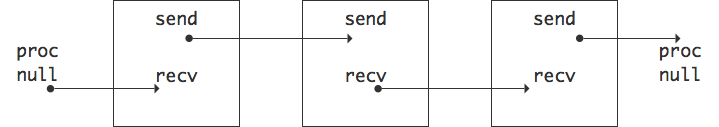
\includegraphics[scale=.6]{sendrecv-actual}
\end{lulu}
\begin{notlulu}
    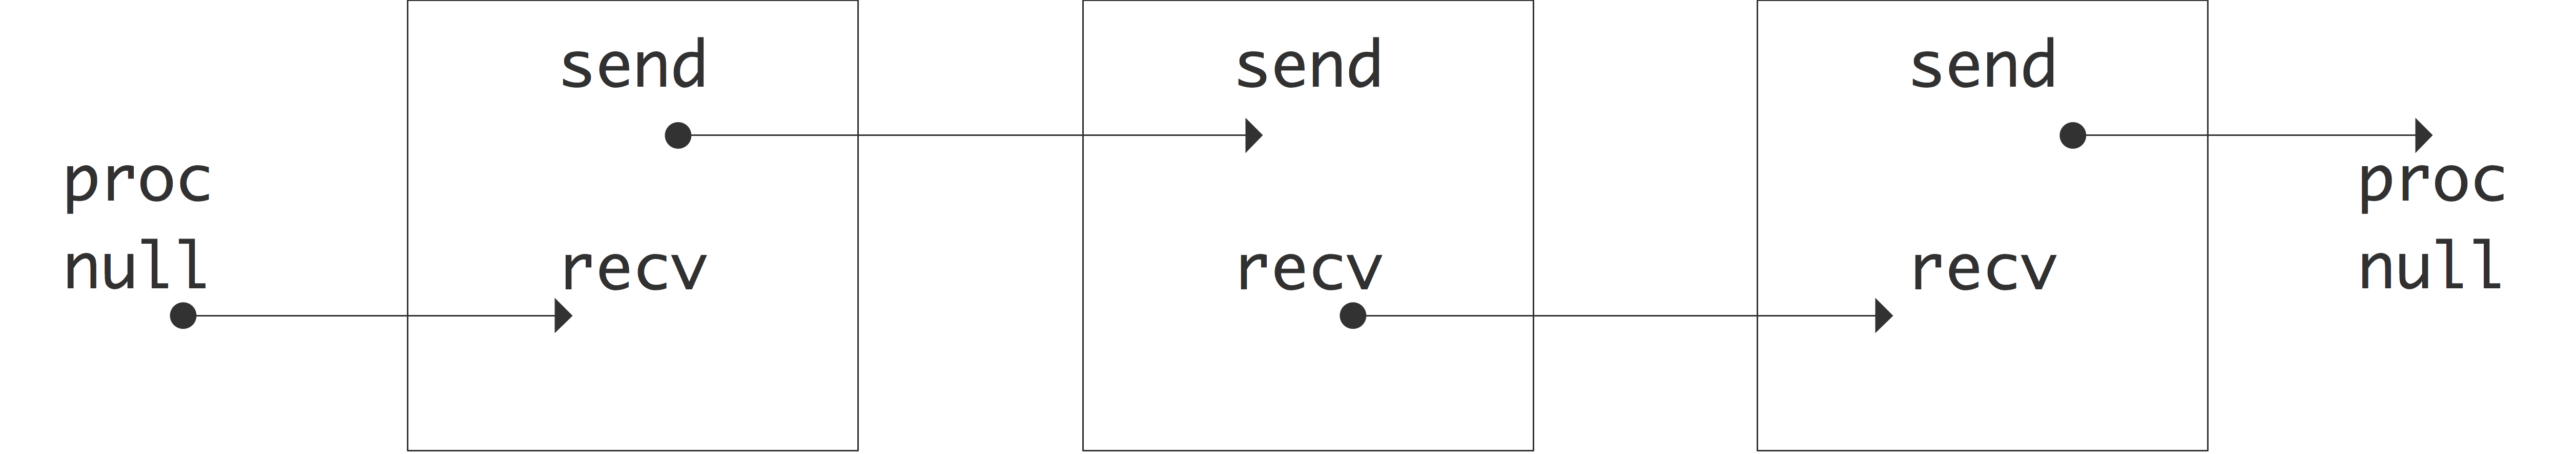
\includegraphics[scale=.09]{sendrecv}
\end{notlulu}
  \caption{An MPI Sendrecv call}
  \label{fig:sendrecv}
\end{figure}
Above you saw some examples that had most processors doing both a send and
a receive, but some only a send or only a receive. You can still use
\n{MPI_Sendrecv} in this call if you use \indexmpishow{MPI_PROC_NULL} for
the unused source or target argument.

If the send and receive buffer have the same size, the routine
\indexmpishow{MPI_Sendrecv_replace} will do an in-place replacement.

\mpiRoutineRef{MPI_Sendrecv_replace}

The following exercise lets you implement a sorting algorithm with the
send-receive call\footnote {There is an \n{MPI\_Compare\_and\_swap}
  call. Do not use that.}.
%
\begin{exercise}
  \label{ex:exchangesort}
\begin{wrapfigure}{r}{3.5in}
  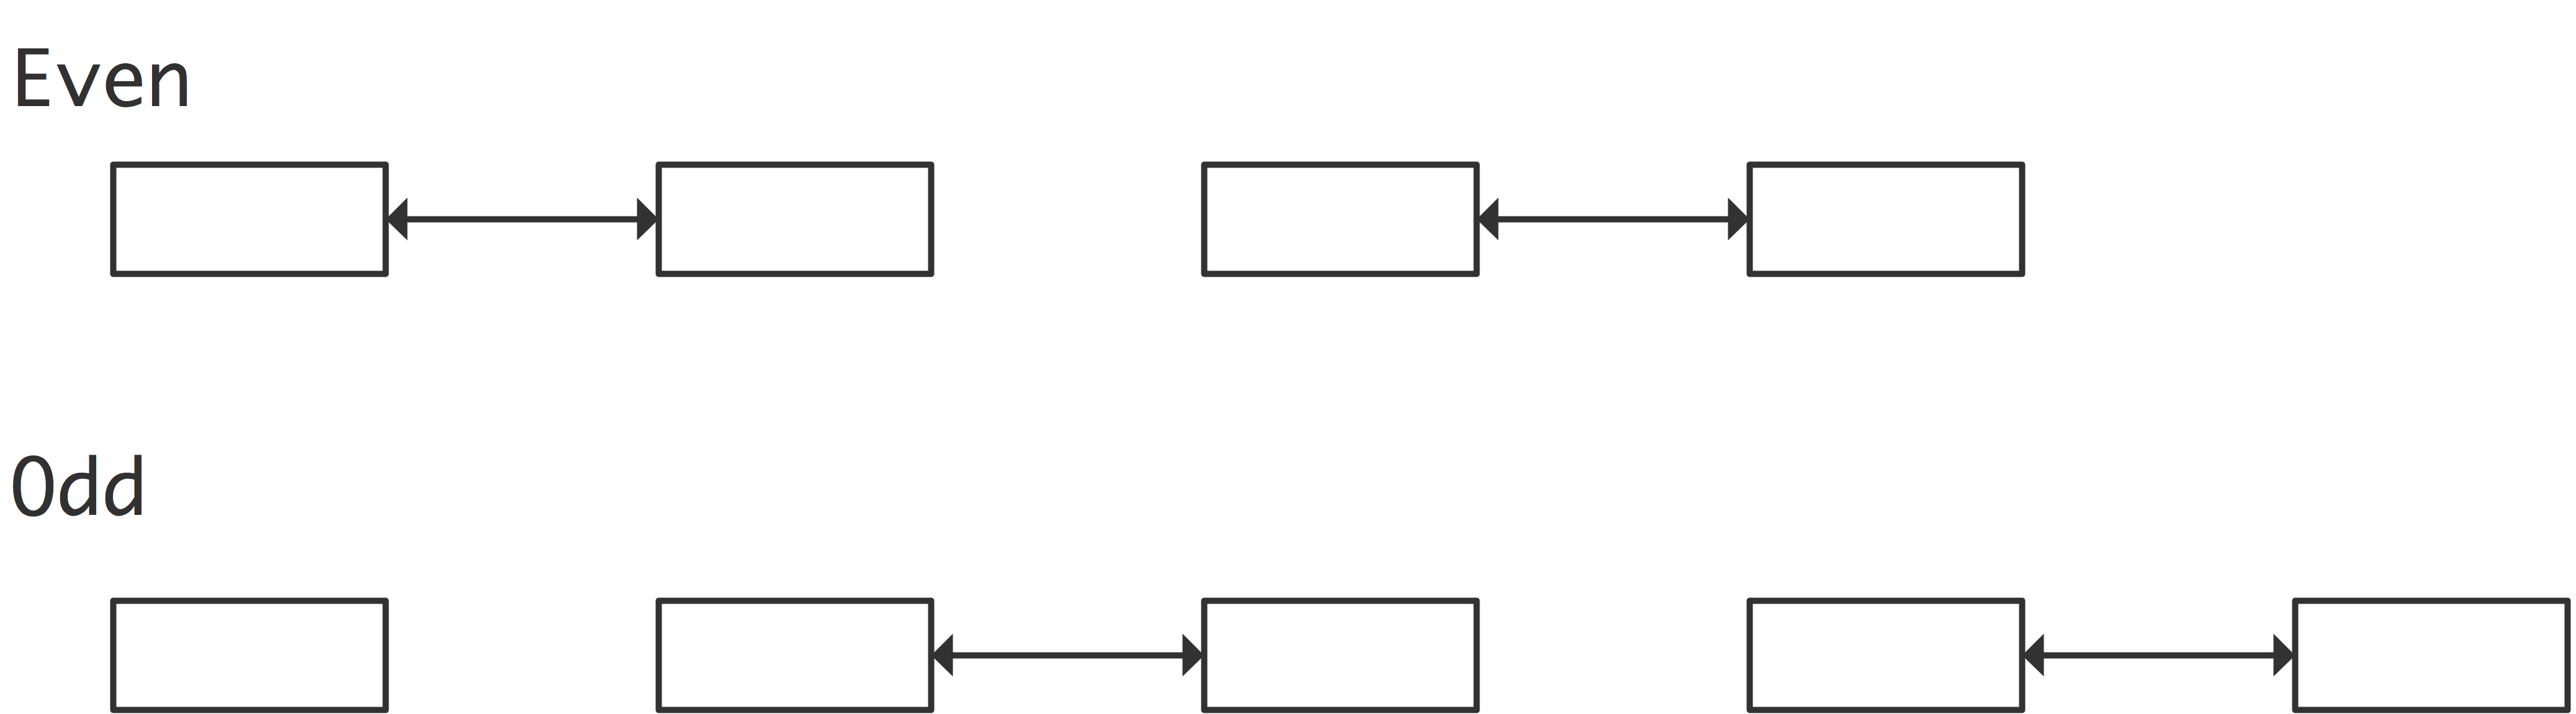
\includegraphics[scale=.06]{swapsort}
\end{wrapfigure}
%
  A very simple sorting algorithm is \indextermsub{exchange}{sort}:
  pairs of processors compare data, and if necessary exchange. The
  elementary step is called a \indexterm{compare-and-swap}: in a pair
  of processors each sends their data to the other; one keeps the
  minimum values, and the other the maximum.
  For simplicity, in this exercise we give each processor just a single number.

  The exchange sort algorithm is split in even and odd stages, where
  in the even stage, processors $2i$ and $2i+1$ compare and swap data,
  and in the odd stage, processors $2i+1$ and $2i+2$ compare and swap.
  You need to repeat this $P/2$ times, where $P$~is the number of
  processors.

  Implement this algorithm using \n{MPI_Sendrecv}. (You can use
  \n{MPI_PROC_NULL} for the edge cases, but that is not strictly necessary.)
  Use a gather call to print the global state of the distributed array
  at the beginning and end of the sorting process.
\end{exercise}

\Level 1 {Message status}
\label{sec:mpi-status}
\index{message!status|(}

Above, you saw that \indexmpishow{MPI_Receive} has a `status' argument
of type \indexmpishow{MPI_STATUS} that \indexmpishow{MPI_Send} lacks.
(The various \indexmpishow{MPI_Wait...}  routines also have a status
argument; see section~\ref{sec:mpi-nonblock}.) The reason for this
argument is
as follows.

In some circumstances the recipient may not know all details of a
message when you make the receive call, so MPI has a way of querying
the \emph{message status}
\begin{itemize}
\item If you are expecting multiple incoming messages, it may be most
  efficient to deal with them in the order in which they arrive. So,
  instead of waiting for specific message, you would specify
  \indexmpishow{MPI_ANY_SOURCE} or \indexmpishow{MPI_ANY_TAG} in
  the description of the receive message. 
  Now you have to be able to ask `who did this message come from,
  and what is in it'.
\item Maybe you know the sender of a message, but the amount of data
  is unknown. In that case you can overallocate your receive buffer,
  and after the message is received ask how big it was, or you can
  `probe' an incoming message and allocate enough data when you find
  out how much data is being sent.
\end{itemize}

\mpiRoutineRef{MPI_Status}

Using the \indexmpishow{MPI_ANY_SOURCE} specifier. We retrieve the
actual source from the \indexmpishow{MPI_Status} object through the
\indexmpishow{MPI_SOURCE} field.
%
\verbatimsnippet{anysource}
%
\verbatimsnippet{anysourcep}

If you are not interested in
the status information, you can use the values
\indexmpishow{MPI_STATUS_IGNORE} for \indexmpishow{MPI_Wait} and
\indexmpishow{MPI_Waitany},
or \indexmpishow{MPI_STATUSES_IGNORE} for \indexmpishow{MPI_Waitall}
and \indexmpishow{MPI_Waitsome}.

The \indexmpishow{MPI_Status} object
is a structure with the following
freely accessible members:
%
\mpiRoutineRef{MPI_SOURCE}
%
\mpiRoutineRef{MPI_TAG}
%
\mpiRoutineRef{MPI_ERROR}

In section~\ref{sec:mpi-source} we mentioned the master-worker model
as one opportunity for inspecting the \indexmpishow{MPI_SOURCE} field
of the \indexmpishow{MPI_Status} object.

There is also
opaque information: the amount of data received can be retrieved by a
function call to \indexmpishow{MPI_Get_count}.
%
\mpiRoutineRef{MPI_Get_count}
%
This may be necessary since the \n{count} argument to \n{MPI_Recv} is 
the buffer size, not an indication of the actually expected number of
data items.

If you 
precisely know what is going to be sent, the status argument tells you 
nothing new. Therefore, there is a special value \indexmpishow{MPI_STATUS_IGNORE}
that you can supply instead of a status object, which tells MPI that the 
status does not have to be reported. For routines such as \indexmpishow{MPI_Waitany}
where an array of statuses is needed, you can supply \indexmpishow{MPI_STATUSES_IGNORE}.

\label{message!status|)}

object describing the data that was received.
%

\endinput

\Level 1 {Examples}

\mpiexample{MPI_Send}

A regular ping-pong operation with \indexmpishow{MPI_Send} and
\indexmpishow{MPI_Recv}. We repeat the experiment multiple times to
get a reliable measurement of the time taken.
%
\verbatimsnippet{pingpong}
%
\verbatimsnippet{pingpongp}
%
\verbatimsnippet{pingpongpp}

\mpiexample{MPI_Recv}


\mpiexample{MPI_Sendrecv}

We set up a ring structure and use \n{MPI_Sendrecv} to communicate
between pairs.
%
\verbatimsnippet{sendrecvring}

